\section{Data}
To train our models, a dataset derived from 309 robot exploring simulations will be used.
The dataset is composed of 4613 datapoints. Each datapoint is represented as a tuple $$(M, a, ate, are)$$
where:
\begin{enumerate}
    \item $M\in[0,255]^{n\times n}$: robot maps representend as $n \times n$ grayscale maps that a robot has
    obtained during its navigation. Some examples are reported in Figure \ref{fig:floorplans};
    \item $a\in\mathbb{R}^+$: area measurements of the floorplan images, expressed in $m^2$;
    \item $ate\in\mathbb{R}^+$: ATE values, expressed in $m$;
    \item $are\in\mathbb{R}^+$: ARE values, expressed in $rad$;
\end{enumerate}

\noindent
Maps were obtained incrementally during all robot exploration, starting from the beginning and extracting the
current slam robot map every 30 seconds wall time until the environment was fully explored. The choice to use incremental maps is due to the fact that we wants to estimate ATE and ARE online, while the robot is navigating.

The dataset has been randomly partitioned into training, validation, and test sets with proportions 70\%, 15\%, and 15\% respectively.

\begin{figure}[H]
        \centering
        \begin{minipage}{0.32\textwidth}
            \centering
            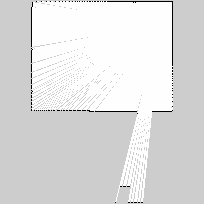
\includegraphics[width=\linewidth]{figures/floorplan1.png}
        \end{minipage}
        \hfill
        \begin{minipage}{0.32\textwidth}
            \centering
            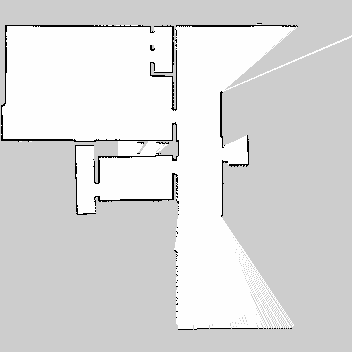
\includegraphics[width=\linewidth]{figures/floorplan2.png}
        \end{minipage}
        \hfill
        \begin{minipage}{0.32\textwidth}
            \centering
            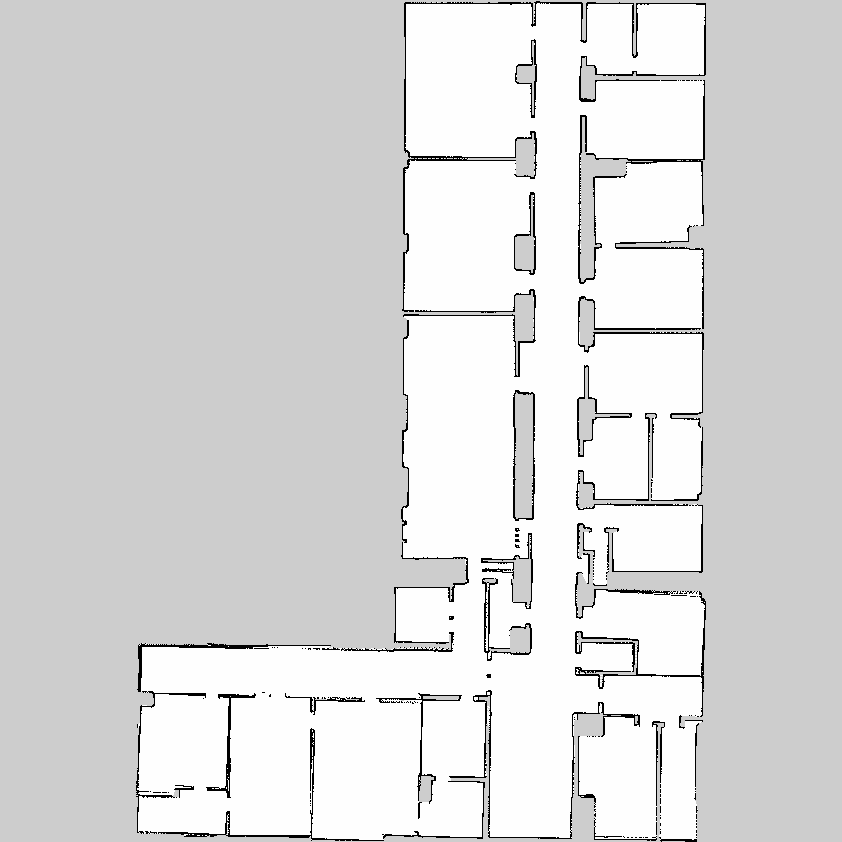
\includegraphics[width=\linewidth]{figures/floorplan3.png}
        \end{minipage}
        \captionsetup{width=0.95\linewidth}
        \caption{Examples of grayscale floorplan images used as input; the white pixels represent the
        free area, the black pixels the obstacles and the gray pixels the unknown area.\label{fig:floorplans}}
    \end{figure}

\subsection{Data preprocessing}

Evaluating the APE values shows that they are mainly distributed towards zero, with a significant presence of 
outliers, especially for ATE values. Figure \ref{fig:dataBoxPlot} shows the histograms with highlighted the 
0.99-quantile and the first value such that its Z-score is greater or equal to 3.5; the Z-score of a number 
$x$ is $Z = \frac{x-\overline{x}}{\sigma}$ where $\overline{x}$ is the mean and $\sigma$ the standard deviation.
\begin{figure}[H]
    \centering
    
\includegraphics[width=\linewidth]{figures/APE_box.pdf}
    \vspace{-2em}
    \captionsetup{width=0.95\linewidth}
    \caption{Box plot of the ATE (top) and ARE (bottom) values with log scale on the y axe; is also shown the 0.99-quantile (red line) and 
    the first value with a z-score equal to 3.5 (blue line).\label{fig:dataBoxPlot}}
\end{figure}

\noindent
To facilitate our models to learn each quantity, the following strategies have been applied:
\begin{itemize}
    \item Outliers cleaning: data points with ATE or ARE values above the $0.99$-quantile or with a Z-score 
    greater than or equal to 3.5 have been removed to reduce the impact of extreme outliers. 113 datapoints
    were removed;
    \item Logarithmic rescaling: due to the skewed distribution of ATE and ARE, a logarithmic transformation
        has been applied to these values to reduce the effect of large values and improve model learning; let
        $x$ be the interested value to be rescaled, the applied operation is: 
        $$ \log(1+x) $$ where $\log$ is the
        natural logarithm;

    \item Rescaling: after the logarithmic rescaling, a linear rescaling to $[0,1]$ has been applied; let
        $\{x_1,\dots,x_n\}$ be interested values to be rescaled, the applied operation is 
        \begin{equation} \frac{x_i}{\underset{1\leq k \leq n}{\max}x_k} \tag*{i=1,\dots,n} \end{equation}
        \begin{figure}[ht]
            \raggedleft
            \begin{minipage}{0.92\textwidth}
                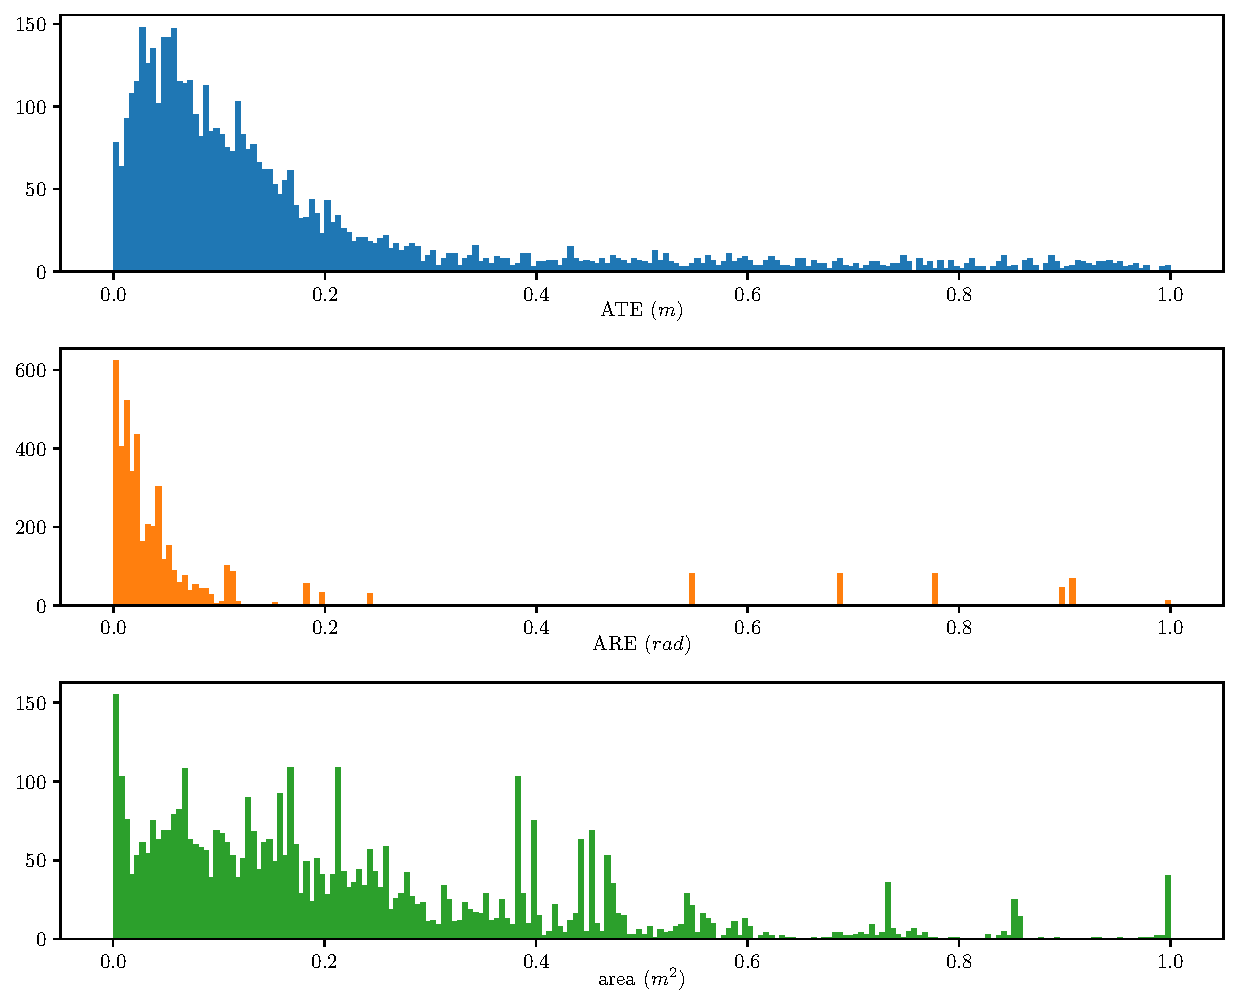
\includegraphics[width=0.9\linewidth]{figures/APE_norm_hist.pdf}
            \end{minipage}
            \vspace{-1em}
            \caption{Dataset values after the log and linear rescaling.\label{fig:datahisttransf}}
        \end{figure}
        Figure \ref{fig:datahisttransf} shows data distribution after all the trasformations.

    \item Image cropping: each map has been cropped to remove unnecessary borders, focusing only on the relevant 
        area to reduce input size and eliminate irrelevant background; the crop is always squared in order to
        mantain this property to all floorplan images. Figure \ref{fig:squaredBox} shows an example of this 
        operation;
        \begin{figure}[H]
            \centering
            \begin{minipage}{0.92\textwidth}
                \hspace{4em}
                \begin{minipage}{0.35\textwidth}
                    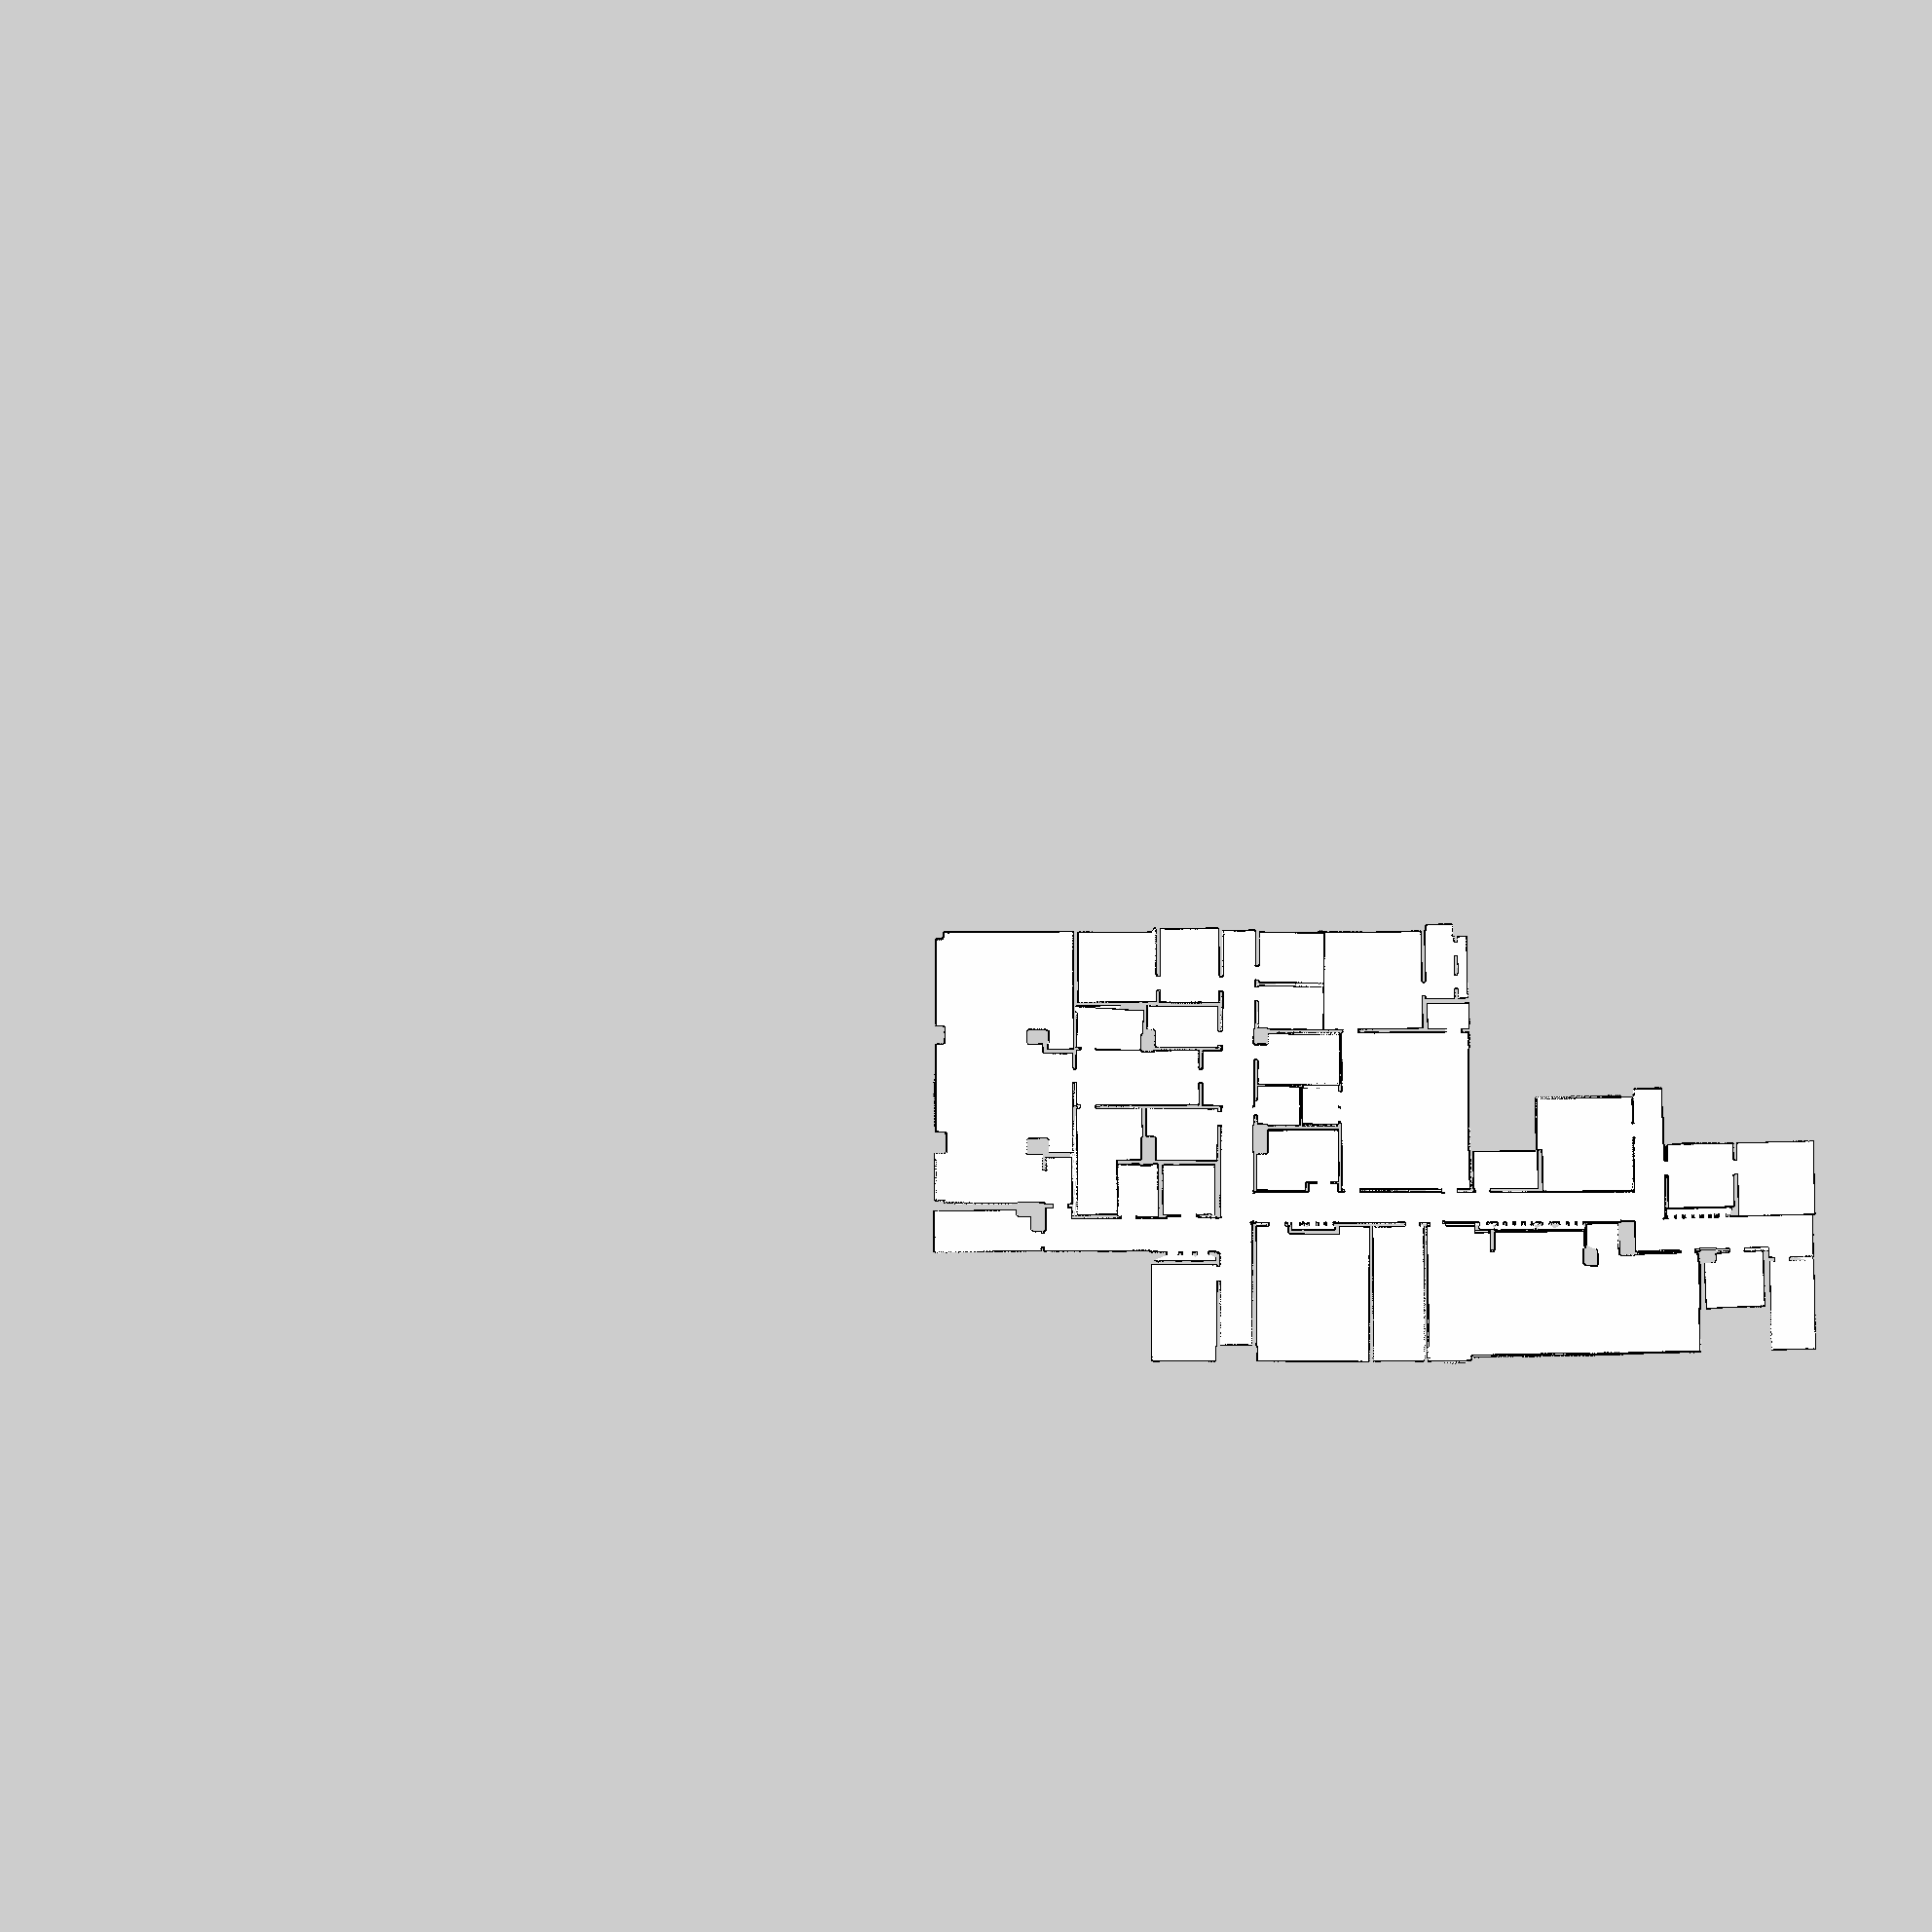
\includegraphics[width=\linewidth]{figures/notSquaredMap.png}
                \end{minipage}
                \hspace{2em}
                \begin{minipage}{0.35\textwidth}
                    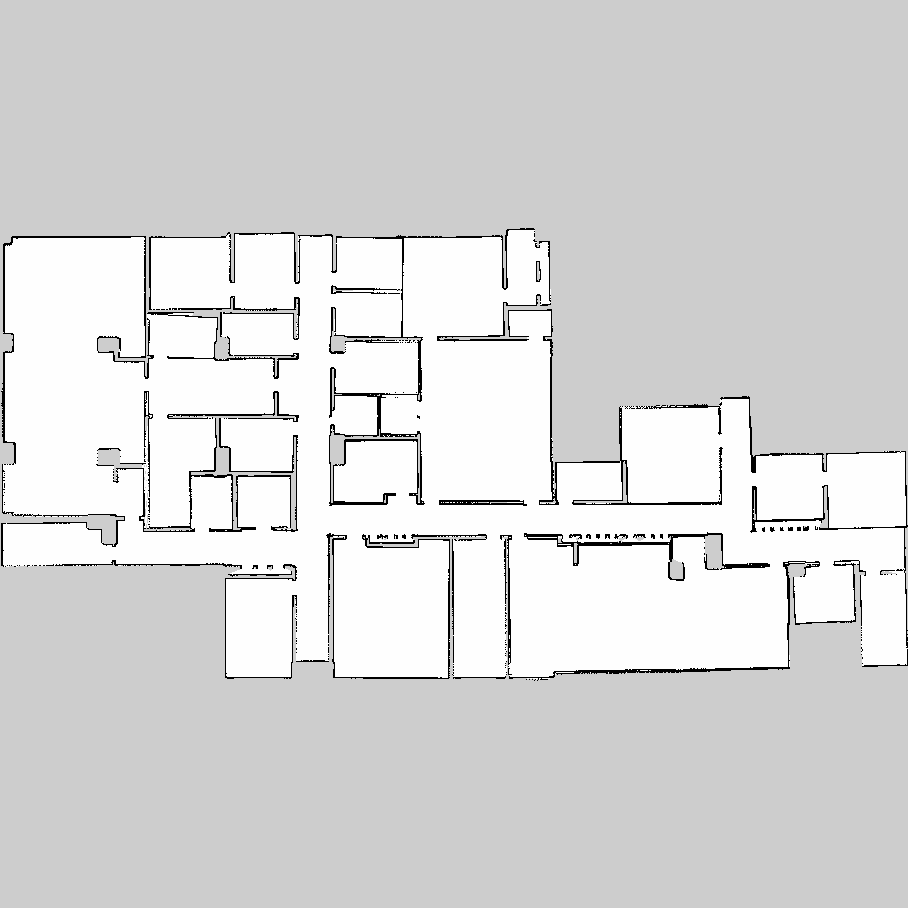
\includegraphics[width=\linewidth]{figures/squaredMap.png}
                \end{minipage}
                \hfill
            \end{minipage}
            \caption{A floorplan (left) and its bounding square crop (right).\label{fig:squaredBox}}
        \end{figure}
    \item Image resizing: each floorplan image is resized to $224 \times 224$ pixels to 
        ensure a uniform input size for the neural network models;
\end{itemize}

\subsection{Data augmentation}
Given the relatively limited size of the dataset, the following data augmentation techniques have been applied to
training set:
\begin{itemize}
    \item Random flip: both horizontal and vertical flips are applied;
    \item Random rotation: random rotation between $0^\circ,90^\circ,180^\circ,270^\circ$ is applied; 
\end{itemize}